\chapter{Repaso de Aritmética, Álgebra y Notación}

En este capítulo introductorio resumiremos la mayoría de las ideas y conceptos básicos de matemáticas que se aprenden en la educación básica. Varios de ellos serán revisados con mucho mayor detalle y en un contexto más amplio, con miras a la matemática pre-universitaria, en los capítulos posteriores.

\section{Teorema fundamental de la aritmética, mcm y mcd}

El {\bf teorema fundamental de la aritmética} establece que todo número natural se \emph{factoriza como producto} de {\bf números primos}: $$n=p_1^{\alpha_1}\cdot p_2^{\alpha_2}\cdots p_k^{\alpha_k}.$$
{\bf Factorizar} es la acción de descomponer un número o una expresión como producto de números más pequeños o expresiones más sencillas, llamados {\bf factores}.

Por ejemplo: 
$$12=2^2\cdot 3,\quad 15=3\cdot 5,\quad 20= 2^2\cdot 5,\quad 36=2^2\cdot 3^2, \quad 49=7^2, \quad 50=2\cdot 5^2, \quad 100=2^2\cdot 5^2, \quad 101=101.$$

$$(x+y)^3=(x+y)(x+y)(x+y)=x^3+3x^2y+3xy^2+y^3, \quad (x-y)^2 =(x-y)(x-y)=x^2-2xy+y^2.$$

$$(x+y+z)^2=(x+y+z)(x+y+z)=x^2+y^2+z^2+3xy+3xz+3yz$$

Dos de las más inmediatas aplicaciones del teorema fundamental de la aritmética es para calcular el {\bf mínimo común múltiplo} $\mathrm{mcm}[n,m]$ y el {\bf máximo común divisor} $\mathrm{mcd}(n,m)$. Para calcularlos, se deben considerar simultáneamente las factorizaciones de ambos números $$n=p_1^{\alpha_1}\cdot p_2^{\alpha_2} \cdots p_k^{\alpha_k}, \quad m=q_1^{\beta_1}\cdot q_2^{\beta_2} \cdots q_k^{\beta_k},$$
donde se vale que algunas $\alpha_i$, $\beta_j, i\neq j$ sean ceros. 

El {\bf máximo común divisor} $$(m,n):= \mathrm{mcd}(n,m):= p_1^{\min\{\alpha_1,\beta_1\}}\cdot p_2^{\min\{\alpha_2,\beta_2\}} \cdots p_k^{\min\{\alpha_k,\beta_k\}}$$ se calcula multiplicando todos los factores primos que aparecen en \emph{ambas} factorizaciones, tomando el \emph{mínimo exponente para cada primo}.

En contraparte, el {\bf minimo comun multiplo} toma los maximos para cada par de exponentes: $$[m,n]:= \mathrm{mcm}(n,m):= p_1^{\max\{\alpha_1,\beta_1\}}\cdot p_2^{\max\{\alpha_2,\beta_2\}} \cdots p_k^{\max\{\alpha_k,\beta_k\}}$$. 

Por ejemplo, la siguiente tabla contiene los valores de $\mathrm{mcd}(n,m)$ para $n,m= 12,15,20,36,49,50,100,101$:
\begin{center}
\begin{tabular}{|c||c|c|c|c|c|c|c|c|c|} 
 \hline
  $m\setminus n$& $12$ & $15$ & $20$ & $36$ & $49$ & $50$& $99$ & $100$ & $101$ \\ 
  \hline
  \hline
  $12$ & $12$ & $3$ & $4$ & $12$ & $1$ & $2$ & $3$ & $4$ & $1$ \\
  \hline
  $15$ & $3$ & $15$ & $5$ & $3$ & $1$ & $5$ & $3$ & $5$ & $1$ \\
  \hline
  $20$ & $4$ & $5$ & $20$ & $4$ & $1$ & $10$ & $1$ & $20$ & $1$ \\
  \hline
  $36$ & $12$ & $3$ & $4$ & $36$ & $1$ & $2$ & $9$ & $4$ & $1$ \\ 
  \hline
  $49$ & $1$ & $1$ & $1$ & $1$ & $49$ & $1$ & $1$ & $1$ & $1$ \\
  \hline
    $50$ & $2$ & $5$ & $10$ & $2$ & $1$ & $50$ & $1$ & $50$ & $1$ \\
  \hline
    $99$ & $3$ & $3$ & $1$ & $9$ & $1$ & $1$ & $99$ & $1$ & $1$ \\
  \hline
    $100$ & $4$ & $5$ & $20$ & $4$ & $1$ & $50$ & $1$ & $100$ & $1$ \\
  \hline
    $101$ & $1$ & $1$ & $1$ & $1$ & $1$ & $1$ & $1$ & $1$ & $101$ \\
  \hline
  \end{tabular}    
\end{center}
Observa que dos números consecutivos no comparten primos, por lo tanto, el $\mathrm{mcd}(n,n+1)=1$. El máximo común divisor juega un rol muy importante en teoría de números.

Por otro lado, el mínimo común múltiplo $\mathrm{mcm}[n,m]$ se construye multiplicando todos los primos que aparecen en \emph{alguna} de las factorizaciones, tomando como exponente el \emph{máximo exponente para cada primo}.


Por ejemplo, la siguiente tabla contiene los valores de $\mathrm{mcm}[n,m]$ para $n,m= 12,15,20,36,49,50,100,101$:
\begin{center}
\begin{tabular}{|c||c|c|c|c|c|c|c|c|c|} 
 \hline
  $m\setminus n$& $12$ & $15$ & $20$ & $36$ & $49$ & $50$& $99$ & $100$ & $101$ \\ 
  \hline
  \hline
  $12$ & $12$ & $60$ & $60$ & $36$ & $588$ & $300$ & $1188$ & $300$ & $1212$ \\
  \hline
  $15$ & $60$ & $15$ & $60$ & $180$ & $735$ & $150$ & $495$ & $300$ & $1515$ \\
  \hline
  $20$ & $60$ & $60$ & $20$ & $180$ & $980$ & $100$ & $1980$ & $100$ & $2020$ \\
  \hline
  $36$ & $36$ & $180$ & $180$ & $36$ & $1740$ & $900$ & $396$ & $900$ & $3636$ \\ 
  \hline
  $49$ & $588$ & $735$ & $980$ & $1740$ & $49$ & $2450$ & $4851$ & $4900$ & $4949$ \\
  \hline
    $50$ & $300$ & $150$ & $100$ & $900$ & $2450$ & $50$ & $4950$ & $100$ & $5050$ \\
  \hline
    $99$ & $1188$ & $495$ & $1980$ & $396$ & $4851$ & $4950$ & $99$ & $9900$ & $9999$ \\
  \hline
    $100$ & $300$ & $300$ & $100$ & $900$ & $4900$ & $100$ & $9900$ & $100$ & $10100$ \\
  \hline
    $101$ & $1212$ & $1515$ & $2020$ & $3636$ & $4949$ & $5050$ & $9999$ & $10100$ & $101$ \\
  \hline
  \end{tabular}    
\end{center}

\begin{ejercicio}
Lista todos los números primos menores que $50$.
\end{ejercicio}

\begin{ejercicio}
Factoriza los siguientes números. 
$$60,\quad 240, \quad 150,  \quad 300, \quad  1000,\quad 1001.$$
\end{ejercicio}

\begin{ejercicio}
Completa las tablas con los $\mathrm{mcd}(n,m)$ (izq.) y $\mathrm{mcm}[n,m]$ (der.)
\end{ejercicio}

\begin{tabular}{|c||c|c|c|c|c|c|} 
 \hline
  $m\setminus n$& $60$ & $150$ & $240$ & $300$ & $1000$ & $1001$ \\ 
  \hline
  \hline
  $60$&  &  &  &  &  &  \\
  \hline
  $150$&  &  &  &  &  &  \\ 
  \hline
  $240$&  &  &  &  &  &  \\ 
  \hline
  $300$&  &  &  &  &  &  \\ 
  \hline
  $1000$&  &  &  &  &  &  \\
  \hline
  $1001$&  &  &  &  &  &  \\ 
  \hline
  \end{tabular}    
  \hspace{1cm}
  \begin{tabular}{|c||c|c|c|c|c|c|} 
 \hline
  $m\setminus n$& $60$ & $150$ & $240$ & $300$ & $1000$ & $1001$ \\ 
  \hline
  \hline
  $60$&  &  &  &  &  &  \\ 
  \hline
  $150$&  &  &  &  &  &  \\ 
  \hline
  $240$&  &  &  &  &  &  \\ 
  \hline
  $300$&  &  &  &  &  &  \\ 
  \hline
  $1000$&  &  &  &  &  &  \\
  \hline
  $1001$&  &  &  &  &  &  \\ 
  \hline
  \end{tabular}    

\begin{ejercicio}
Demuestra que para cualesquiera números enteros $m,n$, se cumple que $$mn=(m,n)[m,n].$$
\end{ejercicio}

\section{Simplificando fracciones y expresiones algebraicas}

Una {\bf fracción} $\frac{n}{d}$ representa una {\bf proporción}. 

Un ejemplo bastante útil para entender fracciones, por la simetría circular de los objetos involucrados y nuestra familiaridad con la acción de partirlos en pedazos iguales, es pensar en rebanadas de pizza o de pastel. 

El {\bf denominador} $d\neq 0$ nos indica en cuántos \emph{pedazos iguales} se cortan las pizzas. El {\bf numerador} nos indica cuántas rebanadas le tocan a una persona (puede que me toque más de una pizza completa $n>d$, o que deba pizzas que no he pagado $n<0$).

Una misma proporción se puede representar de \emph{muchas maneras}. Por ejemplo, obtengo la misma cantidad de pastel si éste se divide en $20$ rebanadas idénticas de las que tomo $4$, a que si el mismo pastel se divide en $10$ rebanadas y tomo $2$. 

    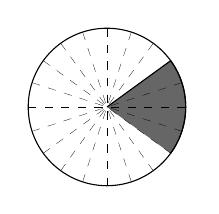
\begin{tikzpicture}
\draw[fill=gray!120] (0,
0) -- +(36:1) arc (36:-36:1);
\draw (0,0) circle [radius=1];
    \foreach \i in {0,...,9} \draw[dashed, black, line width=0.1pt] 
    (18*\i:1) -- (-180+18*\i:1);
\end{tikzpicture}         
\hspace{2cm}
    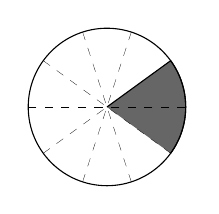
\begin{tikzpicture}
\draw[fill=gray!120] (0,0) -- +(36:1) arc (36:-36:1);
\draw (0,0) circle [radius=1];
    \foreach \i in {0,...,4} \draw[dashed, black, line width=0.1pt] 
    (36*\i:1) -- (-180+36*\i:1);
\end{tikzpicture}         
\hspace{2cm}
    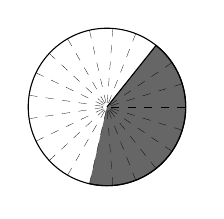
\begin{tikzpicture}
\draw[fill=gray!120] (0,0) -- +(17.1428*3:1) arc (17.1428*3:-17.1428*6:1);
\draw (0,0) circle [radius=1];
    \foreach \i in {0,...,20} \draw[dashed, black, line width=0.1pt] 
    (17.1428*\i:1) -- (0,0);
\end{tikzpicture}
\hspace{2cm}
    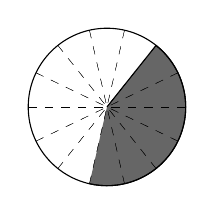
\begin{tikzpicture}
\draw[fill=gray!120] (0,0) -- +(25.7142*2:1) arc (25.7142*2:-25.7142*4:1);
\draw (0,0) circle [radius=1];
    \foreach \i in {0,...,13} \draw[dashed, black, line width=0.1pt] 
    (25.7142*\i:1) -- (-180+25.7142*\i:1);
\end{tikzpicture}

Es decir, $\frac{4}{20}=\frac{2}{10}$ y de la misma manera $\frac{9}{21}=\frac{6}{14}$. Decimos que estas fracciones son {\bf equivalentes}. En general, dos fracciones $\frac{a}{b}, \frac{c}{d}$ son equivalentes si y solo si $a\cdot d=b\cdot c$. 

En el ejemplo anterior $4\cdot 10 = 2 \cdot 20$ y $9\cdot 14 = 6 \cdot 21$.

Hay una cantidad \emph{infinita de fracciones equivalentes} a una fracción dada $\frac{a}{b}$. Por ejemplo, si multiplico el numerador y el denominador por cualquier número $c$ que no sea cero, obtengo una fracción equivalente $\frac{c\cdot a}{c \cdot b}=\frac{a}{b}$. Entonces, por ejemplo $$\frac{2}{3}=\frac{4}{6}=\frac{6}{9}=\frac{8}{12}=\frac{10}{15}=\cdots, \quad \frac{7}{4}=\frac{14}{8}=\frac{21}{12}=\frac{-7}{-4}=\frac{-14}{-8}=\cdots$$

Normalmente, para facilitar cuentas, estamos interesados en la expresión que involucre los números más pequeños. 

Decimos que una fracción $\frac{a}{b}$ se encuentra {\bf simplificada} si el máximo común divisor $\mathrm{mcd}(a,b)=1$. Con esto se logran los numeradores y denominadores más pequeños. 

\begin{ejercicio}
Para cada una de las siguientes fracciones, escribe 5 fracciones equivalentes. Después encuentra la fracción equivalente simplificada.
\end{ejercicio}

\begin{ejercicio}
A continuación se presentan 20 fracciones. Agrúpalas por conjuntos de fracciones equivalentes.
\end{ejercicio}

Recordemos ahora las reglas para realizar operaciones con fracciones.

El caso más simple es el de la suma y resta con fracciones \emph{con el mismo denominador}. Aquí simplemente se tiene que $$\frac{a}{b}+\frac{c}{b}=\frac{a+c}{b},\quad \frac{a}{b}-\frac{c}{b}=\frac{a-c}{b}.$$
Por ejemplo:
$$\frac{3}{12}+\frac{10}{12}=\frac{13}{12},\quad \frac{4}{15}-\frac{6}{15}=\frac{-2}{15}, \quad \frac{8}{7}+\frac{5}{7}=\frac{13}{7},\quad \frac{12}{8}-\frac{5}{8}=\frac{7}{8}$$

Cuando las fracciones \emph{no tienen el mismo denominador}, se tienen que encontrar \emph{fracciones equivalentes con los mismos denominadores}: Por ejemplo

\begin{ejercicio}
Resuelve las siguientes sumas de fracciones con denominadores distintos.
\end{ejercicio}

Para multiplicar dos, tres o más fracciones la regla es sencilla. Simplemente se multiplican todos los numeradores arriba y se multiplican todos los denominadores abajo. $$\frac{a}{b}\cdot\frac{c}{d}=\frac{ac}{bd},\quad \frac{a}{b}\cdot\frac{c}{d}\cdot\frac{e}{f}=\frac{ace}{bdf}, \quad \frac{n_1}{d_1}\cdot\frac{n_2}{d_2}\cdots \frac{n_k}{d_k}=\frac{n_1n_2\cdots n_k}{d_1d_2\cdots d_k}.$$ 

En principio no es necesario buscar fracciones equivalentes, como en la suma, aunque en general es más eficiente trabajar con fracciones simplificadas.

\begin{ejercicio}
¿Cuánto valen la siguiente multiplicación de fracciones: $$\left(\frac{60}{21}\right)\times\left(\frac{1}{33}\right)\times\left(\frac{6}{5}\right)\times \left(\frac{35}{8}\right)?$$
\end{ejercicio}

\begin{ejercicio}
¿Cuánto vale $$\left(\frac{1}{2}\right)\times\left(\frac{2}{3}\right)\times\left(\frac{3}{4}\right)\times\cdots \times\left(\frac{998}{999}\right)\times\left( \frac{999}{1000}\right)?$$
\end{ejercicio}


La división es la operación inversa a la multiplicación, en el sentido de que:

Cuando el numerador y el denominador presentan algún {\bf factor común}, se puede \emph{simplificar la fracción cancelando el factor común}. Por ejemplo $$\frac{a\times c}{b\times c}=\frac{a}{b}, \quad \frac{a\times b\times c\times d \times e}{f \times c\times g \times a }=\frac{b\times d\times e}{f\times g},$$

%Utilizamos la conmutatividad de la muntuplicación para reordenar las fracciones y cancelarlas.

Es importante mencionar que las cancelaciones solo aplican para factores y no para sumas. Por ejemplo, \emph{no se vale} que en la fracción $\frac{a+c}{b+c}$ se cancelen las $c$'s para obtener $\frac{a+c}{b+c}=\frac{a}{b}$.

Cuando de multiplicaciones se trate, ¡se vale cancelar \emph{cualquier cosa que no sea cero}! (números fraccionarios, decimales, irracionales, complejos, etc).

Por ejemplo, la multiplicación:
$$\frac{\pi}{\sqrt{2}}\times \frac{4}{3 \pi}\times \frac{\sqrt{8}}{10}=\frac{\pi \times 4\times \sqrt{8}}{\sqrt{2} \times 3 \times \pi \times 10}.$$ 
me enfrentaría con una situación horrorosa, pues los números $$\pi=3.141592\dots,\quad  \sqrt{2}=1.4142135\dots, \quad \sqrt{8}=2.8284271\dots$$ son \emph{irracionales}. Esto significa que sus expansiones decimales nunca se acaban y nunca se repiten.

Pero, como $\sqrt{8}=\sqrt{4\times 2}=\sqrt{4}\times \sqrt{2}=2\times \sqrt{2}$, ¡puedo cancelar todos los factores irracionales!:
$$\frac{\pi}{\sqrt{2}}\times \frac{4}{3 \pi}\times \frac{\sqrt{8}}{10}=\frac{\pi}{\sqrt{2}}\times \frac{4}{3 \times \pi}\times \frac{2\times \sqrt{2}}{2\times 5}=\frac{\pi \times \sqrt{2}\times 2 \times 4}{\pi \times \sqrt{2}\times 2\times 3\times 5}=\frac{4}{15}.$$

Este truco, aunque sencillo, se utiliza para simplificar cuentas muy frecuentemente, en todas las áreas de las matemáticas.


\begin{ejercicio}
Muestra que si $\frac{a}{b}=\frac{c}{d}$, entonces $\frac{a}{b}=\frac{a+c}{b+d}$.
\end{ejercicio}

\begin{ejercicio}
Muestra que si $\frac{a}{b}=\frac{a+c}{b+d}$, entonces $\frac{a}{b}=\frac{c}{d}$.
\end{ejercicio}

Los dos ejercicios anteriores juntos muestran que la igualdad $\frac{a}{b}=\frac{c}{d}$ se verifica {\bf si y solamente si} $\frac{a}{b}=\frac{a+c}{b+d}$ se verifica.
%ToDO (ver sección ?).

%%%%%%%%%%%%%%%%%%%%%%%%%%%%%%%%%%%%%%%%%%%%%%%%%%%%%%%%%%%%

\newpage

\section{Póngale nombre}

Para organizar mejor un cálculo o una demostración matemática es conveniente \emph{ponerles nombres} a los objetos que deseamos estudiar. Así podemos referirnos a ellos con facilidad y manipularlos para resolverlos, compararlos o estudiarlos.

Se le puede poner nombre a números (naturales, enteros, racionales, etc.), objetos geométricos (ángulos, lados, áreas, circunferencias etc.), conjuntos, funciones y muchos objetos matemáticos más.

Entre otros caracteres, se utilizan frecuentemente en matemáticas: 
\begin{itemize}
    \item letras minúsculas del abecedario: $a,b,c,\dots d, \dots f,g,h, \dots k, \dots m,n, \dots p,q,r, \dots ,x,y,z,$ 
para nombrar números constantes, divisores, funciones, naturales, primos , incógnitas, coordenadas, etc).
    \item letras mayúsculas: $A,B,C,\dots, X,Y,Z$, (para nombrar conjuntos, puntos en el plano, etc).
    \item letras griegas minúsculas: $\alpha$, $\beta$, $\gamma$, $\delta$, $\theta$, etc. (para nombrar ángulos, permutaciones, la constante irracional $\pi=3.141592\dots $, etc). 
    \item símbolos especiales $\mathbb{N}, \mathbb{Z}, \mathbb{Q}, \mathbb{R}, \mathbb{C}$ (para nombrar, respectivamente, a los conjuntos de números naturales, enteros, racionales, reales y complejos). En estas notas, utilizaremos $\mathbb P$, y $\mathbb E$ para denotar a las funciones que calculan la probabilidad de un evento y su valor esperado (en probabilidad). 
\end{itemize}

Sin embargo, estas convenciones no son absolutamente estrictas y tenemos en principio la libertad de elegir el nombre que se nos antoje y que nos parezca más conveniente para un objeto matemático de nuestro interés. 

Supongamos que me piden calcular la suma de los primeros cien números naturales $1+2+3+4+\cdots +98+99+100$. Como al principio no sé cuánto vale, podría llamarle  <<$x$>> a esa suma: $$x:=1+2+3+4\cdots +99+100,$$ para después intentar calcular el valor de $x$. Como dijimos, tenemos absoluta libertad de elegir el nombre y <<$x$>> es solamente una elección de una infinidad de posibilidades.

Al mismo objeto matemático bien le podríamos poner el nombre <<$s$>>, $$s:=1+2+3+4+\cdots+99+100,$$ porque así la letra $s$ me recuerda que se trata de una suma, y le puedo preguntar: <<¿Qué tranza, ése?>>.

Los dos puntos al lado izquierdo del signo igual  $:=$ se utilizan para \emph{nombrar por primera vez a un objeto matemático}. Solamente se utilizan al momento del bautizo. Un vez que mi objeto tiene nombre, los puntos se omiten. Por ejemplo, después de calcular la suma, obtengo que $s=5050$ (ver sig. capítulo).

Los nombres pueden incluir {\bf índices}. Por ejemplo, si ahora me piden calcular el valor de tres sumas, la primera $1+2+3+4+\cdots+9+10$, la segunda $1+2+3+4+\cdots+99+100$ y la tercera $1+2+3+4+\cdots +999+1000$, podría llamarles $$s_1:=1+2+3+4+\cdots+9+10,\quad s_{2}:=1+2+3+4+\cdots+99+100, \quad s_{3}:=1+2+3+4+\cdots +999+1000,$$ para así distinguir entre las tres sumas, manipularlas y calcularlas.

Aunque no sepa el valor específico de $s_1$, $s_2$ y $s_3$ puedo asegurar sin muchos problemas que el primero es menor que el segundo, que a su vez es menor que el tercero y comunicar todo esto de forma práctica y compacta: $$s_1<s_2<s_3.$$

Si así lo quisiera, el nombre puede ser aún más informativo. Por ejemplo, podría llamarles $$s_{10}:=1+2+3+4+\cdots+9+10,\quad s_{100}:=1+2+3+4+\cdots+99+100, \quad s_{1000}:=1+2+3+4+\cdots +999+1000,$$
para que la variable (el <<nombre>>), me indique directamente cuántos números se están sumando.

A veces una notación sofisticada con índices nos puede ser muy útil. En otras ocasiones, por el contrario, la misma notación sofisticada podría resultar tediosa o poco práctica.

De la misma forma que asignamos $$s_{100}:=1+2+3+\dots+99+100,$$ podríamos nombrar al producto de los primeros números <<$\mathrm{perro}_{100}$>>, o: $$p_{100}:=1\times 2\times 3\times \cdots \times 99\times 100.$$

Esta última definición, aunque es válida, sería un despropósito. Los productos de los primeros $n$ enteros positivos son números bastante utilizados en matemáticas, pues aparecen de manera elemental en problemas de combinatoria, álgebra, probabilidad y análisis. Entonces es natural que los matemáticos ya se hayan puesto de acuerdo en cómo llamarles:
$$100!:=1\times 2\times 3\times \cdots \times 99\times 100.$$
El $100!$ se lee <<{\bf cien factorial}>>. Por convención se define $0!:=1$ (ver Sección 2.4).

Por su parte, aunque la suma de los primeros naturales no tiene un nombre por si solo, está determinada por un símbolo bastante estándar en matemáticas, llamado el {\bf coeficiente binomial} $${n\choose k}=\frac{n!}{k!(n-k)!}=\frac{n\times (n-1)\times \cdots \times 3\times2\times1}{k\times(k-1)\times \cdots \times 2\times 1\times (n-k)\times(n-k-1)\times \cdots \times 2\times 1},$$
(casualmente definido en términos de factoriales).

A partir de aquí tenemos que jubilar al símbolo $\times$ como signo de multiplicación. Es mucho mas claro y recomendable escribir $2\cdot 3 = 6$, $(2)(3)=6$, $2(3)=6$, $(2)3=6$, que escribir $2\times 3 = 6$. Sobre todo cuando se escribe a mano, el $\times$ se puede confundir con una letra $x$ 

Como en particular (ver primer capítulo sobre conteo): $$1+2+3+\cdots+n={n+1\choose 2}=\frac{n(n+1)}{2},$$
no hay necesidad de establecer un nuevo símbolo universal para denotar la suma de los primeros $n$ números naturales.

El encontrar buenos nombres para objetos matemáticos es un arte que se perfecciona con el tiempo. La regla dorada es \emph{no repetir el mismo nombre para dos objetos matemáticos distintos}. Si no respetamos esta regla confundiremos de forma terrible quien nos esté leyendo, o peor, \emph{calificando} (y probablemente a nosotros mismos).

\section{Productos notables}

\section{Simplificación de ecuaciones algebraicas (Igualdad)}

\section{Desigualdades}

\section{Notación de conjuntos y funciones}

\section{Conjuntos famosos}

\section{Los números complejos}


%%%%%%%%%%%%%%%%%%%%%%%%%%%%%%%%%%%%%%%%%%%%%%%%%%%%%%%%%%%%
\newpage



%\section{Manipulación de expresiones algebraicas}

%\subsection{Si y solamente si}

%Una expresión súper utilizada en la jerga matemática es el mentado <<si y solamente si>>. Es tan importante y frecuente que se abrevia <<si y solo si>>, <<ssi>> o con el símbolo de relación <<$\Longleftrightarrow$>>. 

%En esta sección explicaremos qué significa eso de <<P si y solamente si Q>>. Al principio este concepto podrá parecer un poco extraño, pero después de varios ejercicios se irá clarificando.

%Para empezar, <<$\Longleftrightarrow$>> no nos resulta completamente ajeno: en los ejercicios \ref{} y \ref{} nos pidieron demostrar exactamente que, para $a,b,c,d\in \mathbb Z$ con $b,d\neq 0$,  \[\frac{a}{b}=\frac{c}{d} \Longleftrightarrow  \frac{a}{b}=\frac{a+c}{b+d}\] 

%ToDo: Breve explicación de ssi.

%Ejemplo 2: Otro?.

%Ejemplo 3: Mediatriz.

%\subsection{Igualdades}

%\subsection{Desigualdades}



